\def\mytitle{IMPLEMENTATION OF BOOLEAN LOGIC IN VAMAN ESP}
\def\myauthor{Naru Soundarya}
\def\contact{narusoundarya2002@gmail.com}
\def\mymodule{Future Wireless Communication (FWC)}
\documentclass[10pt, a4paper]{article}
\usepackage[a4paper,outer=1.5cm,inner=1.5cm,top=1.75cm,bottom=1.5cm]{geometry}
\twocolumn
\usepackage{graphicx}
\graphicspath{{./images/}}
\usepackage[colorlinks,linkcolor={black},citecolor={blue!80!black},urlcolor={blue!80!black}]{hyperref}
\usepackage[parfill]{parskip}
\usepackage{lmodern}
\usepackage{tikz}
%\documentclass[tikz, border=2mm]{standalone}
\usepackage{karnaugh-map}
%\documentclass{article}
\usepackage{tabularx}
\usepackage{circuitikz}
\usetikzlibrary{calc}
\usepackage{enumitem}
\usepackage{amsfonts}
\usepackage{amssymb}
\usepackage{graphicx}
\usepackage{hyperref}
\renewcommand*\familydefault{\sfdefault}
\usepackage{watermark}
\usepackage{lipsum}
\usepackage{xcolor}
\usepackage{listings}
\usepackage{float}
\usepackage{titlesec}
       \usepackage[latin1]{inputenc}
       \usepackage{color}
       \usepackage{array}
       \usepackage{longtable}
       \usepackage{calc}
       \usepackage{multirow}
       \usepackage{hhline}
       \usepackage{ifthen}

\titlespacing{\subsection}{1pt}{\parskip}{3pt}
\titlespacing{\subsubsection}{0pt}{\parskip}{-\parskip}
\titlespacing{\paragraph}{0pt}{\parskip}{\parskip}
\newcommand{\figuremacro}[5]{
    \begin{figure}[#1]
        \centering
        \includegraphics[width=#5\columnwidth]{#2}
        \caption[#3]{\textbf{#3}#4}
        \label{fig:#2}
    \end{figure}
}

\lstset{
frame=single, 
breaklines=true,
columns=fullflexible
}

\def\ifundefined#1{\expandafter\ifx\csname#1\endcsname\relax}
\ifundefined{inputGnumericTable}
\def\gnumericTableEnd{\end{document}}
\else
   \def\gnumericTableEnd{}
\fi
\providecommand{\gnumericmathit}[1]{#1} 
\providecommand{\gnumericPB}[1]%
{\let\gnumericTemp=\\#1\let\\=\gnumericTemp\hspace{0pt}}
 \ifundefined{gnumericTableWidthDefined}
        \newlength{\gnumericTableWidth}
        \newlength{\gnumericTableWidthComplete}
        \newlength{\gnumericMultiRowLength}
        \global\def\gnumericTableWidthDefined{}
 \fi
 \ifthenelse{\isundefined{\languageshorthands}}{}{\languageshorthands{english}}
\providecommand\gnumbox{\makebox[0pt]}
\setlength{\bigstrutjot}{\jot}
\setlength{\extrarowheight}{\doublerulesep}
\setlongtables

\setlength\gnumericTableWidth{%
	98pt+%
	118pt+%
0pt}
\def\gumericNumCols{2}
\setlength\gnumericTableWidthComplete{\gnumericTableWidth+%
         \tabcolsep*\gumericNumCols*2+\arrayrulewidth*\gumericNumCols}
\ifthenelse{\lengthtest{\gnumericTableWidthComplete > \linewidth}}%
         {\def\gnumericScale{1*\ratio{\linewidth-%
                        \tabcolsep*\gumericNumCols*2-%
                        \arrayrulewidth*\gumericNumCols}%
{\gnumericTableWidth}}}%
{\def\gnumericScale{1}}

\ifthenelse{\isundefined{\gnumericColA}}{\newlength{\gnumericColA}}{}\settowidth{\gnumericColA}{\begin{tabular}{@{}p{98pt*\gnumericScale}@{}}x\end{tabular}}
\ifthenelse{\isundefined{\gnumericColB}}{\newlength{\gnumericColB}}{}\settowidth{\gnumericColB}{\begin{tabular}{@{}p{118pt*\gnumericScale}@{}}x\end{tabular}}

\thiswatermark{\centering \put(181,-119.0){\includegraphics[scale=0.13]{iith_logo3}} }
\title{\mytitle}
\author{\myauthor\hspace{1em}\\\contact\\FWC22021\hspace{6.5em}IITH\hspace{0.5em}\mymodule\hspace{6em}ASSIGNMENT}
\begin{document}
	\maketitle
	\tableofcontents
	\section{problem}
 Write the Boolean Expression for the result of the Logic Circuit as shown below:
\begin{figure}[h]
    \centering
    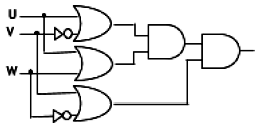
\includegraphics[scale=1]{1.PNG}
     \caption{circuit}
      \label{fig:circuit}
\end{figure}
\section{solution}
    %\caption
    \begin{center}
    ${\boldmath{F}=\boldmath{U}(\boldmath{V}+\boldmath{!W})}$
    \end{center}
	\section{Components}
  \begin{tabularx}{0.48\textwidth} { 
  | >{\centering\arraybackslash}X 
  | >{\centering\arraybackslash}X 
  | >{\centering\arraybackslash}X | }
\hline
 \textbf{Components}& \textbf{Values} & \textbf{Quantity}\\
\hline
Vaman Board&  & 1 \\  
\hline
JumperWires& M-F& 5 \\ 
\hline
Breadboard &  & 1 \\
\hline
USB-C Cable &  & 1 \\
\hline
USB-UART &  & 1 \\
\hline
\end{tabularx}
\section{The steps for implementation:}
\begin{enumerate}
\item Connect the USB-UART pins to the Vaman ESP32 pins according to Table 

\begin{tabular}[c]{%
	b{\gnumericColA}%
	b{\gnumericColB}%
	}
\hhline{|-|-}
	 \multicolumn{1}{|p{\gnumericColA}|}%
	{\gnumericPB{\centering}\gnumbox{{\color[rgb]{0.79,0.13,0.12} VAMAN LC PINS}}}
	&\multicolumn{1}{p{\gnumericColB}|}%
	{\gnumericPB{\centering}\gnumbox{{\color[rgb]{0.79,0.13,0.12} UART PINS}}}
\\
\hhline{|--|}
	 \multicolumn{1}{|p{\gnumericColA}|}%
	{\gnumericPB{\centering}\gnumbox{GND}}
	&\multicolumn{1}{p{\gnumericColB}|}%
	{\gnumericPB{\centering}\gnumbox{GND}}
\\
\hhline{|--|}
	 \multicolumn{1}{|p{\gnumericColA}|}%
	{\gnumericPB{\centering}\gnumbox{ENB}}
	&\multicolumn{1}{p{\gnumericColB}|}%
	{\gnumericPB{\centering}\gnumbox{ENB}}
\\
\hhline{|--|}
	 \multicolumn{1}{|p{\gnumericColA}|}%
	{\gnumericPB{\centering}\gnumbox{TXD0}}
	&\multicolumn{1}{p{\gnumericColB}|}%
	{\gnumericPB{\centering}\gnumbox{RXD}}
\\
\hhline{|--|}
	 \multicolumn{1}{|p{\gnumericColA}|}%
	{\gnumericPB{\centering}\gnumbox{RXD0}}
	&\multicolumn{1}{p{\gnumericColB}|}%
	{\gnumericPB{\centering}\gnumbox{TXD}}
\\
\hhline{|--|}
	 \multicolumn{1}{|p{\gnumericColA}|}%
	{\gnumericPB{\centering}\gnumbox{0}}
	&\multicolumn{1}{p{\gnumericColB}|}%
	{\gnumericPB{\centering}\gnumbox{IO0}}
\\
\hhline{|--|}
	 \multicolumn{1}{|p{\gnumericColA}|}%
	{\gnumericPB{\centering}\gnumbox{5V}}
	&\multicolumn{1}{p{\gnumericColB}|}%
	{\gnumericPB{\centering}\gnumbox{5V}}
\\
\hhline{|-|-|}
\end{tabular}
 \item Flash the following setup code through USB-UART using laptop
\begin{center}
\fbox{\parbox{8cm}{\url{https://github.com/soundaryanaru/FWC_assignments/blob/main/iot/codes/setup/src/main.cpp}}}
\end{center}
\begin{center}
\end{center}
\begin{lstlisting}
svn co https://github.com/soundaryanaru/FWC_assignments/trunk/iot/codes/setup
cd  setup
pio run
pio run -t upload
\end{lstlisting}

after entering your wifi username and password (in quotes below)
\begin{lstlisting}
#define STASSID "..." // Add your network credentials
#define STAPSK  "..."
\end{lstlisting}
in src/main.cpp file
\item You can notice that vaman will be connnected to the network credentials provided above.Connect your laptop to the same network ,You should be able to find the ip address of your vaman-esp on laptop using 
\begin{lstlisting}
ifconfig
nmap -sn 192.168.93.1/24
\end{lstlisting}
where your computer's ip address is the output of ifconfig and given by 192.168.6.x
\item Login to termux-ubuntu on the android device and execute the following commands:
\begin{lstlisting}
proot-distro login debian
cd  /data/data/com.termux/files/home/
mkdir iot
svn co https://github.com/soundaryanaru/FWC-assignments/trunk/iot/codes/ota
cd codes
\end{lstlisting}
\item Assuming that the username is Soundarya and password is nithya@123, flash the following code wirelessly
\begin{center}
\fbox{\parbox{8cm}{\url{https://github.com/soundaryanaru/FWC_assignments/blob/main/iot/codes/ota/src/main.cpp}}}
\end{center}
through 
\begin{lstlisting}
pio run 
pio run -t nobuild -t upload --upload-port ip_addres_of_esp
\end{lstlisting}
where you may replace the above ip address with the ip address of your vaman-esp.
\end{enumerate}
\end{document}








